% Formelsammlung Real Time Programming Languages
%
% Geschrieben im WS 2014/2015 an der TU München
% von Markus Hofbauer und Kevin Meyer für LaTeX4EI
% based on template from www.latex4ei.de
% Kontakt: latex@kevin-meyer.de oder via Kontaktformular auf http://latex4ei.de
% Aktuelle Versionen auf https://makeappdev.github.io/TUM-Projekte/

% Dokumenteinstellungen
% ======================================================================
\documentclass[german]{latex4ei/latex4ei_sheet}

\usepackage[european]{circuitikz}
\usepackage{tabularx}
\usepackage{multirow}
\usetikzlibrary{arrows, calc, intersections, shapes, fit, positioning}

% tabularx definition
\newcolumntype{C}{>{\centering\arraybackslash}X}
\newcolumntype{L}{@{\extracolsep\fill}X}

% Eigene Mathoperatoren
\DeclareMathOperator{\log2}{ld}

% Für code
% \definecolor{COMMENTGREEN}{HTML}{228B22}
% \definecolor{MATLABBACKGROUND}{HTML}{FCFCDC}
\lstset{ %
language=Ada,							% choose the language of the code
% basicstyle=\ttfamily,					% the size of the fonts that are used for the code
% emphstyle=\color{yellow}\ttfalily,
% keywordstyle=\color{blue}\ttfamily,
% stringstyle=\color{magenta}\ttfamily,
% commentstyle=\color{COMMENTGREEN}\ttfamily,
xleftmargin=10.3pt,						% distance to margin left
xrightmargin=-3pt,						% distance to margin right
%linewidth=\widthof{\begin{sectionbox}}}		% this would be better instead of left and right margin
% aboveskip=0.6\baselineskip,
% belowskip=0\baselineskip,
numbers=left,                   			% where to put the line-numbers
% framexleftmargin=1.5em,					% distance to xleftmargin
% numberstyle=\ttfamily\footnotesize,		% the size of the fonts that are used for the line-numbers
% stepnumber=1,							% the step between two line-numbers. If it is 1 each line will be numbered
% numbersep=5pt,							% how far the line-numbers are from the code
% backgroundcolor=\color{MATLABBACKGROUND},	% choose the background color. You must add \usepackage{color}
% showspaces=false,						% show spaces adding particular underscores
% showstringspaces=false,					% underline spaces within strings
% showtabs=false,							% show tabs within strings adding particular underscores
% frame=single,							% adds a frame around the code (Box) (Für top und bottom rule set option to "lines")
% rulecolor=\color{gray},					% color of framebox rule
% tabsize=4,								% sets default tabsize to 2 spaces
% captionpos=b,							% sets the caption-position to bottom
breaklines=true,						% sets automatic line breaking
breakatwhitespace=false,					% sets if automatic breaks should only happen at whitespace
escapeinside={\%*}{*)}					% if you want to add a comment within your code
}

% SI-Einheiten
\DeclareSIUnit\voltampere{VA}
\DeclareSIUnit\var{Var}
\DeclareSIUnit\newtonmeter{Nm}
\DeclareSIUnit\voltsecond{Vs}
\DeclareSIUnit\amperesecond{As}

% Nicht neuen, sondern alten Vector benutzen
\let\newvec = \vec
\let\vec = \oldvec

% Weitere Definitionen
\renewcommand{\ggT}[1]{\ensuremath{\operatorname{ggT}\left\{#1\right\}}}

% Title
\title{Real Time Programming Languages}
\author{Markus Hofbauer und Kevin Meyer}
\myemail{latex@kevin-meyer.de}
\mywebsite{https://makeappdev.github.io/TUM-Projekte/}

% Dokumentbeginn
% ======================================================================
\begin{document}

\IfFileExists{git.id}{\input{git.id}}{}
\ifdefined\GitRevision\mydate{\GitNiceDate\ (git \GitRevision)}\fi

\maketitle

\section{General}
\begin{sectionbox}
\subsection{Real Time System}
System or device, that has to satisfy certain timing constraints while functioning.\\
Hard timing constraints for safety critical systems.

\subsection{Programming Models}
\subsubsection{Synchronous Programming Model}
\begin{itemize}
\item model based on programs reacting to events in zero time
\item output based on input is computed immediately
\item implementation: program approximates synchrony by computing a reactor to an event before the next event occurs (ensured by the compiler)
\item no scheduler is necessary
\end{itemize}

\subsubsection{Scheduled Programming Model}
\begin{itemize}
\item program consits of processes, threads, taks
\item scheduler determines which part runs at which time
\item compiler only implements functionality
\item runtime system (scheduler) implements the scheduling
\end{itemize}

\subsubsection{Time Triggered Model}
\begin{itemize}
\item computation takes a fixed non zero amount of time
\item event safety $\Rightarrow$ time safety, but the other way does not hold
\end{itemize}

\subsection{Layers of reactive program}
\begin{itemize}
\item interface: tasks care of input reception and output production
\item reactive kernel: implements logic ot the system
\item data handling layer: perform computaion requested by kernel
\end{itemize}
\end{sectionbox}

\section{Esterel}
\begin{sectionbox}
\begin{emphbox}
	Synchronous Language
\end{emphbox}
reacting to events in zero time ("`instantaneously"'), i.e,
based on the \mbox{\textbf{synchrony hypothesis:}}
\begin{itemize}
\item reaction takes no time w.r.t.\ environment
\item subprocesses take no time w.r.t.\ other subprocesses
\item interprocess communication takes no time
\item statements take time if they say so: await$\ldots$, every$\ldots$
\end{itemize}

\subsection{Esterel in General}
\begin{tablebox}{ll}
\multicolumn{1}{c}{\textbf{Advantage}} & \multicolumn{1}{c}{\textbf{Disadvantage}}\\
\cmrule
model of time & limited flexibility (no dynamic memory)\\
deterministic & limited tool support\\
easy to analyze & semantically not easy for programmer\\
translateable to HW description & implementation is not efficient\\
much easier to verify formally & paradigm doesn't fit for all problems\\
\end{tablebox}

\subsubsection{Signals}
\textbf{Signal coherence rules:}
\begin{itemize}
\item by default: absent
\item if emitted: present
\item can be both: no
\item multiple values per cycle: no
\item propagation of changes: instantaneous
\end{itemize}
\textbf{Internal Signals:}
\begin{itemize}
\item have a limited scope which lies within a module, i.e., is not externally visible
\item can be seen as "`local"' inputs and outputs
\item same semantics as interface signals
\item useful for letting parallel threads interact ("`$||$"')
\end{itemize}
\end{sectionbox}

\begin{sectionbox}
\subsubsection{Loops}
loops are always bounded, means the body of a loop must take time. otherwise: instantaneous loop $\Rightarrow$ invalid

\subsubsection{?-operator}
\begin{itemize}
\item applies to valued signals and sensors
\item their value of the current tick can be obtained with the ?-operator, e.g.: \texttt{O(?I)} assigns the value of \texttt{I} to \texttt{O}
\end{itemize}

\subsubsection{pre-operator}
\begin{itemize}
\item "`timeshift"' in Esterel
\item \texttt{pre()} returns the value of valued signals from when they were previously present (i.e., not from the
previous tick!), e.g.: \mbox{\texttt{O(pre(?I))} assings the previous value of \texttt{I} to \texttt{O}}
\end{itemize}

\subsubsection{Variables}
\begin{itemize}
\item the only thing that do not fall under the signal coherence rules (i.e., they can take multiple values per tick and the order of statements does matter)
\item cannot be used as signal expressions (i.a.: \texttt{abort, present, $\ldots$}), and cannot be shared between concurrent threads
\item scope is defined explicitely with the keywords \texttt{in} (opens scope) and \texttt{end} (closes scope)
\end{itemize}

\subsubsection{Modules/Renaming}
comparable to functions in C, but modules have no parameters, instead use renaming $\Rightarrow$ \texttt{run} can replace signals, variable or assign constants
\end{sectionbox}

\begin{sectionbox}
\subsubsection{Important Shorthands}
\begin{tablebox}{p{3cm}p{3.5cm}}
\textbf{Derived Statement} & \textbf{Kernel Statements}\\ \cmrule
\texttt{halt} & \texttt{loop pause end}\\
\texttt{sustain s} & \texttt{loop emit s; pause end}\\
\texttt{present s then p} & \texttt{present s then p else nothing end}\\
\texttt{await s} & \texttt{trap T in loop pause; present s then exit T end end loop end}\\
\texttt{await immediate s} & \texttt{trap T in loop present s then exit T end; pause end loop end}\\
\texttt{suspend p when immediate s} & \texttt{suspend present s then pause end; p when s}\\
\texttt{abort p when (immediate) s} & \texttt{trap T in suspend p when (immediate) s; exit T || await (immediate) s; exit T; end}\\
\texttt{weak abort p when (immediate) s} & \texttt{trap T in p; exit T || await (immediate) s; exit T; end}\\
\texttt{loop p each s} & \texttt{loop abort p; halt when s end loop}\\
\texttt{every (immediate) s do p end} & \texttt{abort (immediate) s; loop p each s}\\
\end{tablebox}
\end{sectionbox}

\begin{sectionbox}
\subsection{Logical Correctness}
A signal is logically correct, if there exists exactly one status (present or absent) for it that respects the signal coherence law.\\
There are two properties which a signal can exhibit:
\begin{enumerate}
\item \textbf{deterministic}: it has $\le 1$ coherent state
\item \textbf{reactive}: it has $\ge 1$ coherent state
\end{enumerate}
Consequently, a logically correct signal is both determinstic and reactive.

\begin{cookbox}{Logical Correctness Check}
	\item Assume Siganl $s$ is present and check hypothesis
	\item Assume Siganl $s$ is absent and check hypothesis
	\item Repeat step 1 and 2 for all signals (input and output)
	\item Logical Correct if number of correct hypothesis $ = 1$
\end{cookbox}
A program, that is logical correct has exactly one globally coherent state and is much simpler to debug and analyze.
\end{sectionbox}

\begin{minipage}{.49\columnwidth}
\begin{lstlisting}
-- not reactive
module M:
	output O;
	present O then
		nothing;
	else
		emit O;
	end present;
end module;
\end{lstlisting}
\end{minipage}
\begin{minipage}{.49\columnwidth}
\begin{lstlisting}
-- not deterministic
module M:
	output O;
	present O then
		emit O;
	else
		nothing;
	end present;
end module;
\end{lstlisting}
\end{minipage}

\begin{sectionbox}
\subsection{Model Checking/Functional Verification}
\textbf{Formal} proof of functional correctness of a program.
\begin{itemize}
\item Two main properties to check:
\begin{itemize}
\item \textbf{safety:} "`something bad never happens"'
\item \textbf{liveness:} "`something good eventually happens"'
\end{itemize}
\item Specifying Properties:
\begin{itemize}
\item \textit{state formula}: property is element of AP (propositional logic), e.g., Airbus must never go to parking mode unless
weight on wheels (WoW)
\item \textit{path formula:} defines a sequence of states, e.g., when the pilot hits brakes, it has to start braking within $n$ cycles
\end{itemize}
\item Checking the Specification
\end{itemize}
\begin{cookbox}{Module Checking in Esterel}
	\item write an observer module in Esterel, that runs in parallel to your program under analysis (PUA)
	\item compile Esterel to hardware description and run \texttt{xeve}
	\item \texttt{xeve} answers "`possibly emitted"' or "`possibly not emitted"' for every checked output from the observer
\end{cookbox}
\end{sectionbox}

\section{Processor Architecture}
\begin{sectionbox}
\subsection{Single/Multi-Cycle Processors}
\subsubsection{Single-Cycle}
\begin{itemize}
\item clock cyle is determined by the longest path in the machine
\item Advantage: design is easier
\end{itemize}

\subsubsection{Multi-Cycle}
\begin{itemize}
\item implementation: break up instructions into steps, each such step executes in 1 clock cycle
\item different instructions require different number of clock cycles
\item more efficient and less hardware
\end{itemize}

\subsection{Pipelines}
\begin{itemize}
\item relevant for WCET, because hazards will cause timing anomalies.
\item Used in all modern processors, to keep every portion of the processor busy with some instruction.
\item hazards and resulting stalls will not let us reach ideal speedup
\end{itemize}

\subsection{Hazards}
\subsubsection{Data Hazards}
\begin{itemize}
\item Read-after-Write (RaW)
\item Write-after-Write (WaW)
\item Write-after-Read (WaR)
\item Read-after-Read (RaR)
\end{itemize}

\subsubsection{Structural Hazard}
More than one instruction needs the same resource at the same time.

\subsubsection{Control Hazard}
A conditional jump (e.g., \texttt{if} ) took place, which was not expected. Now we have the wrong instruction in the pipeline.

\subsubsection{Avoiding Hazards}
\begin{itemize}
\item \textbf{Data Hazards:} The compiler
\begin{itemize}
\item must take care, that there is "`enough time"' between two instructions
\item could also re-arrange the instructions, such that an instruction is computed much earlier than needed.
\end{itemize}
\item \textbf{Structural Hazards:} depend on the ISA and processor architecture. MIPS does not have them.
\item \textbf{Control hazards:} can be reduced, but not avoided. The processor tries to predict what branches ("`if"'s) are taken
\end{itemize}
\end{sectionbox}

\begin{sectionbox}
\subsubsection{Living with the remaining hazards}
\begin{itemize}
\item \textbf{stalling:} For data and structural hazards. Entire pipeline is suspended, until the critical instruction is completed
\item \textbf{flushing:} For control hazards. Entire pipeline is cleared. It is loaded thereafter with the correct instructions.
\item \textbf{bubbling:} For data and structural hazards. Processor inserts bubbles (\texttt{nop} , `"no operation'") into the pipeline. Bubbles do nothing but delay the upcoming instructions.
\end{itemize}

\subsection{Memory Hierachy}
memory closer to CPU is faster but smaller
\begin{center}
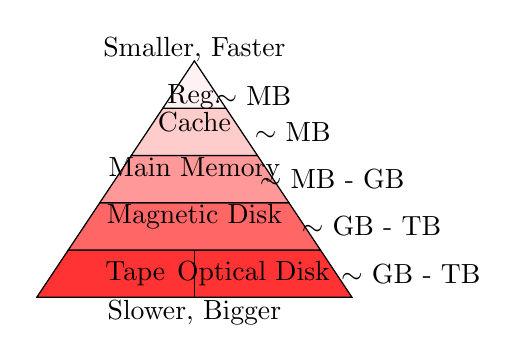
\begin{tikzpicture}[scale=.5,every node/.style={scale=1}]

	\coordinate (L) at (-4,0);
	\coordinate (R) at (4,0);
	\coordinate (O) at (0,6);
	\coordinate (L02) at ($ (L)!.2!(O) $);
	\coordinate (R02) at ($ (R)!.2!(O) $);
	\coordinate (L04) at ($ (L)!.4!(O) $);
	\coordinate (R04) at ($ (R)!.4!(O) $);
	\coordinate (L06) at ($ (L)!.6!(O) $);
	\coordinate (R06) at ($ (R)!.6!(O) $);
	\coordinate (L08) at ($ (L)!.8!(O) $);
	\coordinate (R08) at ($ (R)!.8!(O) $);

	\draw (L) -- (R) -- (O) -- cycle;
	\filldraw[fill=red!80!white, draw=black] (L) -- (R) -- (R02) -- (L02) -- cycle;
	\draw ($(L)!.5!(R)$) -- ($(L02)!.5!(R02)$);
	\node(C02) [fit={(L) (R) (R02) (L02)}] {};
	\draw(C02)++(-1.5,0) node {Tape};
	\draw(C02)++(1.5,0) node {Optical Disk};
	\draw(C02)++(5.5,0) node {$\sim$ GB - TB};
	\draw(C02)++(0,-1) node {Slower, Bigger};

	\filldraw[fill=red!60!white, draw=black] (L02) -- (R02) -- (R04) -- (L04) -- cycle;
	\node(C04) [fit={(L02) (R02) (R04) (L04)}] {Magnetic Disk};
	\draw (C04)++(4.5,0) node {$\sim$ GB - TB};

	\filldraw[fill=red!40!white, draw=black] (L04) -- (R04) -- (R06) -- (L06) -- cycle;
	\node(C06) [fit={(L04) (R04) (R06) (L06)}] {Main Memory};
	\draw (C06)++(3.5,0) node {$\sim$ MB - GB};

	\filldraw[fill=red!20!white, draw=black] (L06) -- (R06) -- (R08) -- (L08) -- cycle;
	\node(C06) [fit={(L06) (R06) (R08) (L08)}] {Cache};
	\draw (C06)++(2.5,0) node {$\sim$ MB};

	\filldraw[fill=red!5!white, draw=black] (L08) -- (R08) -- (O) -- cycle;
	\node(C08) at (0,5.1) {Reg.};
	\draw (C08)++(1.5,0) node {$\sim$ MB};
	\draw (C08)++(0,1.2) node {Smaller, Faster};

\end{tikzpicture}

\end{center}
\end{sectionbox}

\begin{sectionbox}
\subsection{Caches}
\begin{itemize}
\item Relevant for WCET, because hits and misses have different timing.
\item Every level of the memory hierachy can be regarded as a "`cache"'.
\begin{itemize}
\item \textbf{cache hit:} You find the data that you are looking for being in the cache
\item \textbf{cache miss:} Data you are looking for is not in this cache, you have to get it from the next lower level. This takes a lot of time!
\end{itemize}
\end{itemize}

\subsubsection{Direct-mapped caches}
\begin{itemize}
\item if you know the address of your data (which you always do), then you know exactly in which place of the cache it could be
\item this means, you do not have to search the cache for your data (it's fast!)
\item but it wastes the precious cache space (think of modulo$\ldots$)
\end{itemize}

\subsubsection{Associative Cache}
\begin{itemize}
\item if you know the address of your data, then still there is a (limited) number of places in the cache, where it could be
\item you have to look in all those places (it's slower!)
\item but you use your cache much better
\end{itemize}

\subsubsection{Locality}
if an item is referenced:
\begin{itemize}
\item temporal locality: it will tend to be referenced soon
\item spacial locality: nearby will tend to be referenced soon
\end{itemize}

\subsubsection{Cache Calculations}
\begin{tablebox}{ll}
Blocksize & $BS$\\
address space & $AS$\\
way set-associative cache & $w$\\
\cmrule
Number of blocks & $NB = size/BS$\\
number of sets & $NS = NB/w$\\
number of bits for offset field & $WO = \log2(BS)$\\
number of bits for index field & $WI = \log2(NS)$\\
number of bits for tag field & $WT = AS - WO - WI$\\
\end{tablebox}
\begin{center}
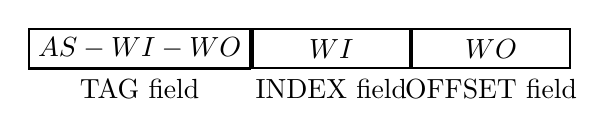
\begin{tikzpicture}[scale=.5,every node/.style={scale=1},node distance=0cm]

\tikzstyle{cache}=[rectangle,draw,thick,minimum width=2cm,minimum height=0.5cm];

\node(INDEX) [cache] {$WI$};
\node [below= of INDEX] {INDEX field};
\node(OFFSET) [cache, right= of INDEX] {$WO$};
\node [below= of OFFSET] {OFFSET field};
\node(TAG) [cache, left= of INDEX] {$AS - WI - WO$};
\node [below= of TAG] {TAG field};

\end{tikzpicture}

\end{center}
\end{sectionbox}

\vfill

\section{WCET}
\begin{sectionbox}
\subsection{WCET Analysis}
Determine how long your code takes in the worst case to complete a certain procedure, to verify the synchrony hypothesis and to perform a schedulability analysis (when multiple programs run in parallel: does each of them finish in time?)

\begin{cookbox}{WCET Analysis using IPET/ILP}
\item \textbf{cross-compile:} for a MIPS-based-processor
\item \textbf{disassemble:} get the assembler code for analysis
\item \textbf{find basic blocks (BB):} group instructions that do not branch/jump (straight line of code with only one enterence and exit point)
\item \textbf{generate control flow graph (CFG):} assembly from 2. turned into a directed graph
\item \textbf{derive structural constraints:} read-off from CFG $\rightarrow$ "`such-that"'-equations for ILP
\item \textbf{add user constraints:} e.g., logical constraints. "`This loop will not run more than $x$ times."'
\item \textbf{Feed ILP (Integer Linear Programming) solver:} objective fcn + constraints go in, the block counts come out ($x_i$), together with the obj. fcn. value, which is WCET
\end{cookbox}

\subsubsection{Definition WCET}
The WCET is the maximum possible execution time a program or procedure can need for completion, considering all possible inputs, all possible internal states/execution paths and assuming uninterrupted processing time. It depends on the specific program and the specific processor it is running on.

\subsection{Compiling Esterel}
Esterel can be compiled to
\begin{itemize}
\item \textbf{finite state machine:} signal not in states; very fast, but long code
\item \textbf{netlist-based compilation (default):} boolean logic circuits; scales well, but very inefficient
\item \textbf{control-flow:} scales well, fast, but bad causality, rarely used
\end{itemize}

\subsection{l(ine)-Blocks}
\begin{itemize}
\item l-block: maximum sequence of code within a basic block such that when the first instruction of the l-block is accessed, either the whole l-block is in the cache, or none of its contents is in the cache
\item A basic block $B_i$ is partitioned into l-blocks $B_{i,1}, B_{i,2},\ldots, B_{i,n}$
\item The execution times of an l-block $B_{i,j}$ are given by $c^\text{hit}_{i,j}$ and $c^\text{miss}_{i,j}$
\end{itemize}
\begin{emphbox}
	WCET = $\sum\limits_{i=1}^N\sum\limits_{j=1}^{n_i} c_{i,j}^\text{hit}x_{i,j}^\text{hit} + c_{i,j}^\text{miss}x_{i,j}^\text{miss}$
\end{emphbox}

\subsection{WCET analysis with caches}
\begin{emphbox}
	WCET = $\underset{x^\text{hit}, x^\text{miss}}{\text{max}}\sum\limits_{i=1}^N c_i^\text{hit}x_i^\text{hit} + c_i^\text{miss}x_i^\text{miss}$
\end{emphbox}

\subsection{Safety}
\begin{itemize}
\item\textbf{event-safety:} in each state of a trace at most a single process action is enabled
\item\textbf{time-safety:} all tasks complete before their output is read
\item\textbf{space-safety:} scheduler doesn't choose unfinished part to execute, when it's shared variable are not yet written
\end{itemize}
\end{sectionbox}

\section{Ada}
\begin{sectionbox}
\begin{emphbox}
	Scheduled Model Language
\end{emphbox}
Real time is the physical time as observed in the external environment.

\subsection{Ada in Gerneral}
\begin{tablebox}{ll}
\multicolumn{1}{c}{\texttt{Ada}} & \multicolumn{1}{c}{\texttt{C++}}\\
\cmrule
\texttt{if then ; else ;} & \texttt{if ; else ;}\\
\texttt{case when (when others)} & \texttt{switch case (default)}\\
\texttt{loop} & \texttt{for}\\
\texttt{while loop} & \texttt{while}\\
\texttt{Records} & \texttt{struct}\\
\texttt{Access} & \texttt{Pointer}\\
\texttt{Generics} & \texttt{Templates}\\
\end{tablebox}

\subsubsection{Difference to C}
\begin{itemize}
\item harder to compile, but less bugs after
\item once it compiles, it works
\item harder to mix data types
\item programmer has to think harder $\rightarrow$ better code
\end{itemize}

\subsection{Tasking}
A task runs concurrently to the rest of the Ada program (=thread) (main program is also a task)
\end{sectionbox}

\begin{sectionbox}
\subsection{Ravenscar Profile}
\begin{itemize}
\item Full Determinism, easier schedulability analysis, memory boundness
\item task are:
\begin{itemize}
\item \textit{time-triggered} (periodic) (released by a single \texttt{delay until})
\item \textit{event-triggered} (sporadic) (released by a single protected entry e.g., to realize interrupts)
\end{itemize}
\item no task hierachies, no rendvous, static task set
\item all entries have capacity of one task
\end{itemize}

\subsubsection{Schedulability Analysis}
process to show, whether all tasks can keep their deadlines.\\
task $:= (P,e,d)$ (with $P = $ Period, $e = $ WCET, $d = $ Deadline) schedulable if:

\begin{emphbox}
	$u = \sum\limits_{i = 1}^{n} \frac{e_i}{P_i} \le n \left(\sqrt[n]{2} - 1 \right)$
\end{emphbox}

\subsubsection{Scheduling Policy}
\begin{itemize}
\item Fixed priority preemption scheduling with immediate priority inheritance and static CPU assingment
\item tasks with highest priority always runs
\item protected objects get ruling priority, which is higher than all other prioritys
\item call inherits priority of protected objects
\end{itemize}
\end{sectionbox}

\end{document}
